\subsection*{SIR -- агентная модель}
\addcontentsline{toc}{subsection}{SIR -- агентная модель}

\textbf{Задание:}\\
Реализовать и проанализировать модель распространения инфекционного заболевания посредством агентного моделирования.\\

\textbf{Решение:}\\
Изначально необходимо создать популяцию людей в размере -- 1000 человек, в непрерывном пространстве, имеющую упорядоченный тип расположения и случайный тип сети с двумя связями. (Рисунок \ref{fig:sir1})
\begin{figure}[h]
	\centering 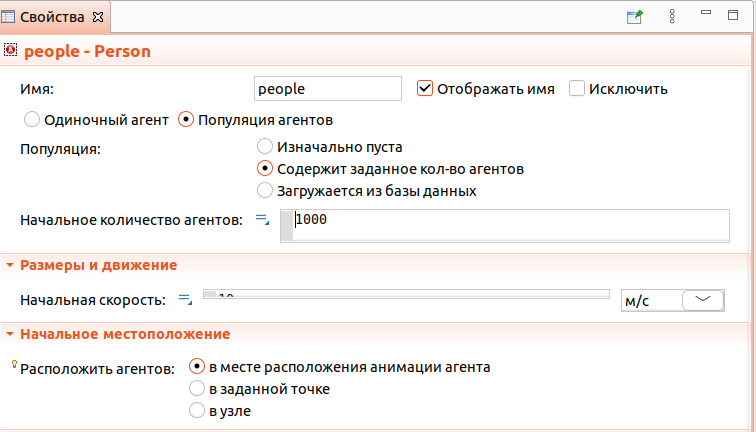
\includegraphics[scale=0.5]{sir1}
	\caption{Настройка агентов модели}
	\label{fig:sir1}
\end{figure}

Далее для всех агентов указываются количество дней, требуемое на восстановление, количество контактов и вероятность заразиться. После задания необходимых параметров модели было решено перейти описанию диаграммы состояний для конкретного агента в популяции. (Рисунок \ref{fig:sir2})
\begin{figure}[h]
	\centering 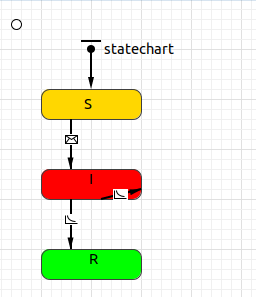
\includegraphics[scale=0.4]{sir2}
	\caption{Описание диаграммы состояний конкретного агента в популяции}
	\label{fig:sir2}
\end{figure}

\newpage

В приведённой выше диаграмме человек может находиться в состояниях:
\begin{enumerate}[topsep=0pt,itemsep=-1ex,partopsep=1ex,parsep=1ex]
	\item когда человек здоров и может заразиться;
	\item когда человек заразился и болеет;
	\item когда человек выздоровел и уже не может заразиться.\\
\end{enumerate}

Переход из первого состояние во второе происходит на основе получения сообщения, отправка сообщения заражённым агентом осуществляется с интенсивностью, равной вероятности заразиться умноженной на количество контактов. Переход из состояния, когда человек болеет в состояние выздоровления происходит согласно интенсивности, равной единице делёной на количество дней, требуемых на восстановления после заболевания данной болезнью.\\

Для начала распространения инфекции необходимо инфицировать нескольких агентов в начале симуляции. (Рисунок \ref{fig:sir3})
\begin{figure}[h]
	\centering 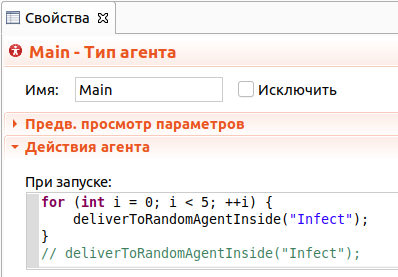
\includegraphics[scale=0.4]{sir3}
	\caption{Инфецирование нескольких агентов на начальной стадии}
	\label{fig:sir3}
\end{figure}

Также был проведёт сбор статистики по числу агентов, которые находятся в рассмотренных выше состояниях для того, чтобы на графиках проанализировать текущую ситуацию модели и как данная модель отличается от рассмотренной ранее. (Рисунок \ref{fig:sir4})
\begin{figure}[h]
	\centering 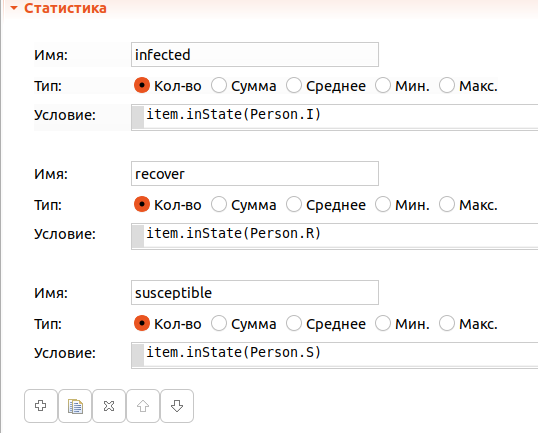
\includegraphics[scale=0.3]{sir4}
	\caption{Сбор статистики по каждому агенту}
	\label{fig:sir4}
\end{figure}

\newpage

Если запустить данную модель, то получим схожую картину, которая была когда мы рассматривали системную-динамику. (Рисунок \ref{fig:sir5})
\begin{figure}[h]
	\centering 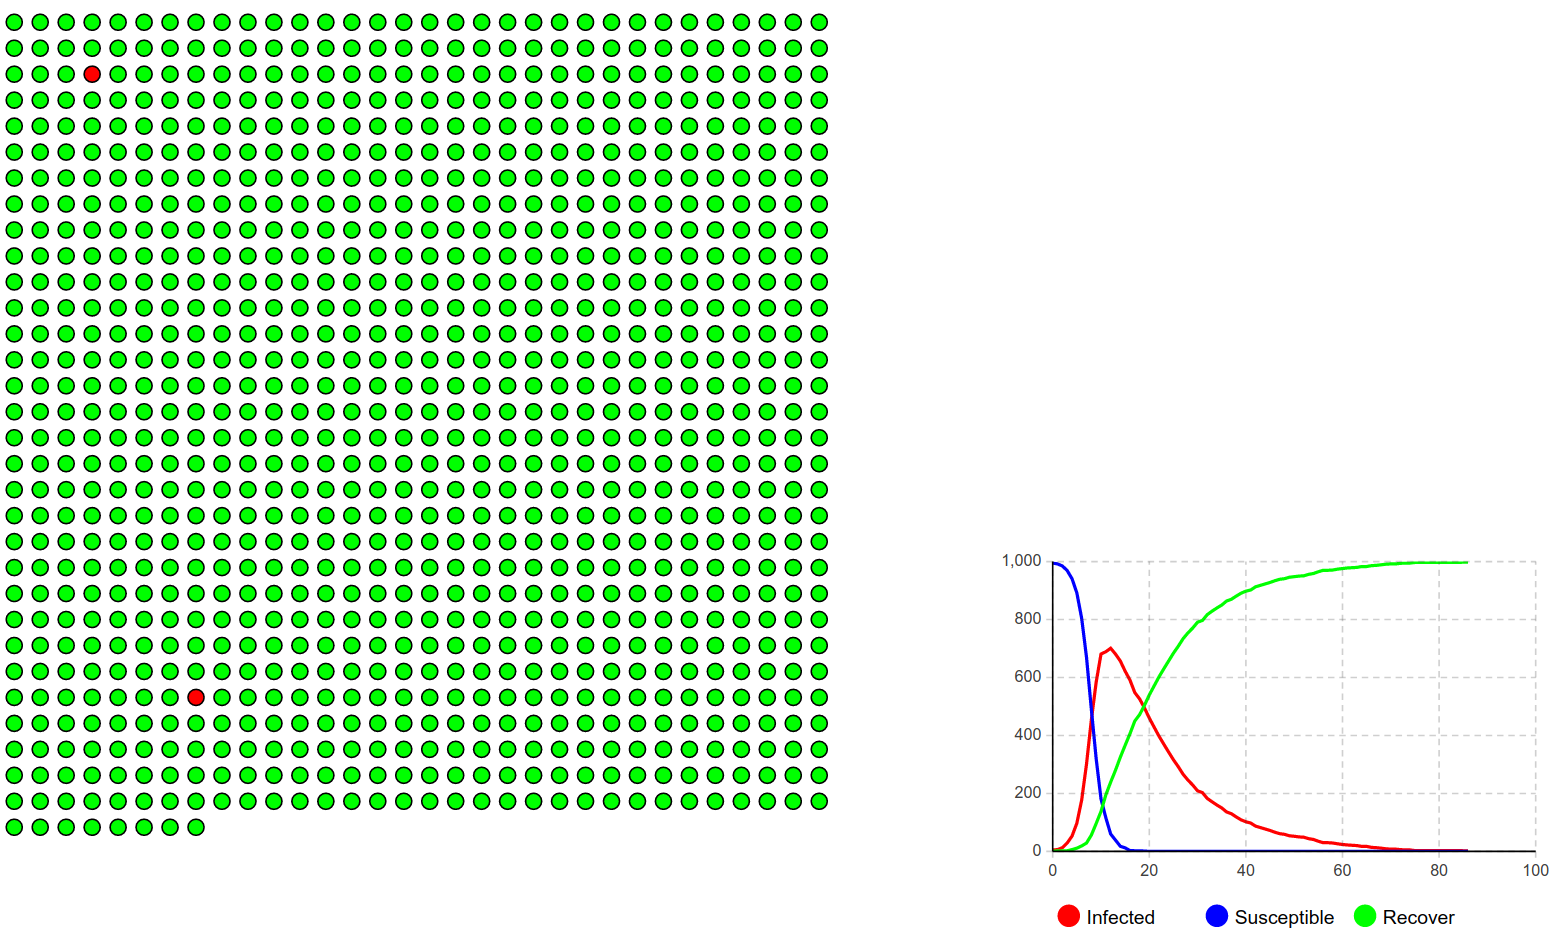
\includegraphics[scale=0.3]{sir5}
	\caption{Процесс моделирования}
	\label{fig:sir5}
\end{figure}

Таким образом, посредством агентного моделирования была реализована модель распространения инфекций.